\chapter{AI Component Design}
\label{chap:ai-component-design}

\section{Business Context \& AI integration}
\label{sec:business_context_ai_integration}
\begin{figure}[h]
    \centering
    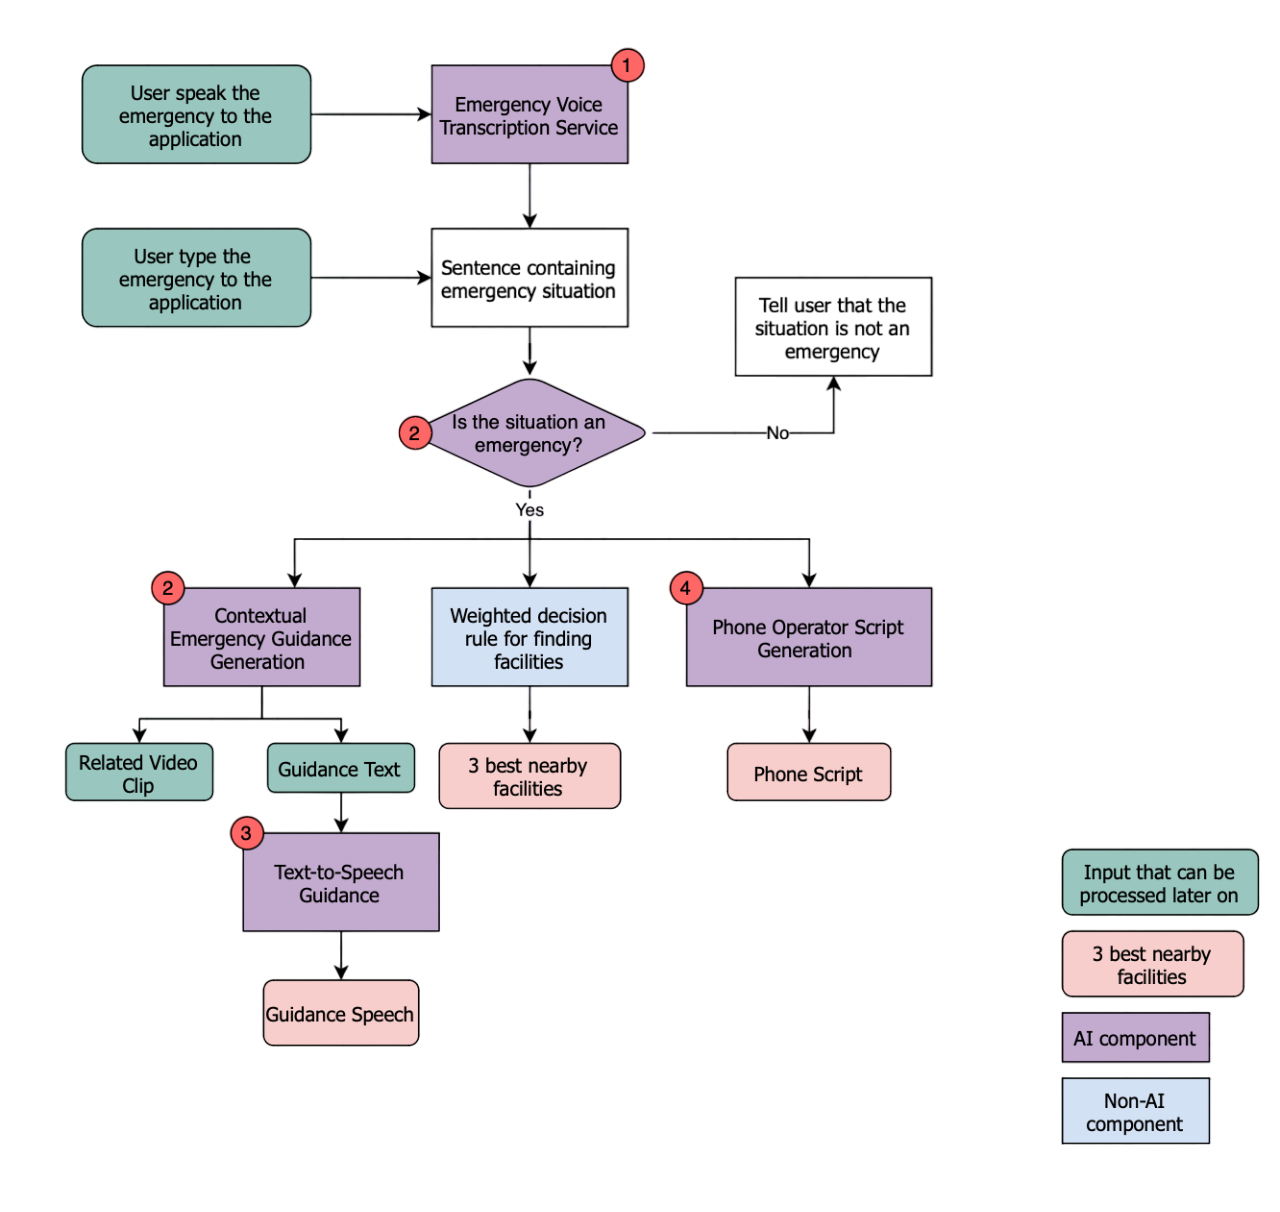
\includegraphics[width=0.9\textwidth]{/flows/business-workflow.png}
    \caption{Business workflow including AI components and non-AI component part}
\end{figure}
\medskip

AI components that will be used in the application:

\subsection{Emergency Voice Transcription Service}
\label{subsec:ai_comp_transcription_service}
In moments of crisis, individuals often find it significantly more challenging to type coherently than to speak. AI-driven STT addresses this by allowing users to verbally describe their emergency. This task is suitable for AI because real-world emergency speech is extraordinarily complex; it can be spoken rapidly under stressful situations, contain strong emotions, and occur in environments with background noise—all factors that make rule-based systems impractical.\\
\indent Furthermore, the nuances of the Thai language, including tones and regional variations, add another layer of complexity that AI models are better equipped to learn and interpret.\\
\indent While perfect transcription is the goal, an initial system might accept an accuracy of more than 80\% of words that are correctly captured. Because even the texts are not 100\% right, the AI model that will processed on this transcribed text will eventually be able to understand the context and give the accurate information to the users.

\subsection{Contextual Emergency Guidance Generation}
\label{subsec:ai_comp_guidance_generation}
When facing an emergency, individuals often don't know the correct immediate actions to take and may be too panicked to search for reliable information.\\
\indent This AI component will assess the situation described by the user, whether it’s through transcribed speech or direct text input and determine if it constitutes an emergency, and then generate specific, actionable guidance with related video clips from the internet. The suitability of AI, such as a specific-to-giving-guidance Large Language Model (LLM), for this task stems from the immense scale and complexity of potential emergency scenarios. Each type of emergency has numerous variables and requires tailored responses that are difficult, if not impossible, to generate with predefined rules. An LLM can process the user's description, understand the context, and provide relevant instructions.\\
\indent For this AI model, the tolerance for error in the guidance provided is extremely low. False or misleading information in a life-or-death situation is unacceptable, so the factual accuracy of the guidance must approach 100\%.

\subsection{Text-to-speech for guidance (TTS)}
\label{subsec:ai_comp_tts}
During high-stress events, users may find it difficult to read and process long text information. Offering an option for users to listen to the guidance instead of reading it can significantly improve understanding and user experience.\\
\indent AI-powered TTS is ideal here because modern neural TTS models can produce highly natural, clear, and appropriately toned speech in Thai, which is far superior to robotic-sounding alternatives and beneficial to calm and effective understanding in a crisis.\\
\indent While the core message must be perfectly conveyed, some minor imperfections that do not affect clarity might be acceptable, aiming for a high level of naturalness and digestibility, maybe above an 80-90\% threshold as perceived by users.

\subsection{Phone operator generation}
\label{subsec:ai_comp_phone_operator}
When users need to contact official emergency services or specific facilities, they may struggle to clearly and concisely convey all necessary information, especially if they are disoriented or panicked, or have difficulty pinpointing their location.\\
\indent This AI component will generate a personalized, structured script in Thai, containing all critical details for the user to read to the operator. AI is well-suited for this because it can dynamically get information such as the nature of the emergency (derived from earlier inputs) and the user's precise current location (obtained via device GPS) and use them to produce an effective message.\\
\indent The accuracy of the information within this script—especially location, type of emergency, and number of people involved—must be near 100\%, as this information is crucial for an effective emergency response by the authorities.


\section{Goal Hierarchy}
\label{sec:goal_hierarchy}
For each AI component, the goal hierarchy will be listed as follows:

\subsection{Emergency Voice Transcription Service}
\label{subsec:goal_voice_transcription}
\begin{itemize}
    \item \textbf{System Goal:} Reliably and rapidly transcribe a user's spoken description of their emergency situation into Thai text, providing an intuitive and easy-to-use voice input interface.
    \item \textbf{User Goal:} To quickly and easily communicate their emergency to the application using their voice, without the need for typing, especially when under stress. Evaluate by collecting user feedback.
    \item \textbf{AI Model Goal:} To accurately convert spoken Thai words into text, demonstrating robustness against background noise, emotional speech, and varied accents (within Central Thai focus). Evaluated by using Word Error Rate (WER) which has to be below 20\% (WER $<$ 20\%) in noisy conditions and below 10\% (WER $<$ 10\%) in quieter conditions. The data collected for evaluating will come from transcribed diverse test sets of Thai speech recorded in various situations.
\end{itemize}

\subsection{Contextual Emergency Guidance Generation}
\label{subsec:goal_guidance_generation}
\begin{itemize}
    \item \textbf{System Goal:} To provide users with clear, accurate, actionable, and contextually appropriate step-by-step emergency guidance in Thai and choose the right video for the user, immediately after an emergency is identified. This will be evaluated by the overall system success rate in delivering relevant guidance (target $>$98\% based on expert review of simulated scenarios), time-to-display guidance from input submission (target $<$3 seconds), and UI/UX ratings for clarity and presentation of guidance (target $>$4/5 via user surveys).
    \item \textbf{User Goal:} To quickly understand what to do (and what not to do) to ensure their safety and manage the emergency situation effectively. This will be evaluated through user surveys on the guidance provided (target $>$90\% correct understanding of critical steps), perceived usefulness surveys (target $>$4.5/5), and user-reported confidence scores after receiving guidance (target $>$4/5).
    \item \textbf{AI Model Goal:} To correctly classify the type and severity of the emergency (whether it’s an emergency or not) based on textual input and generate accurate, relevant, and complete guidance with correct video clip. This will be evaluated by accuracy and safety of guidance content , relevance score (target $>$4.5/5 based on user ratings), completeness score (target $>$4.5/5 ensuring all critical steps are included, rated by experts), and, for internal classification step, an emergency type classification F1-score of $>$0.95. Evaluation data will come from response guidance data set from trusted sources.
\end{itemize}

\subsection{Text-to-speech for guidance}
\label{subsec:goal_tts_guidance}
\begin{itemize}
    \item \textbf{System Goal:} To audibly deliver the generated emergency guidance to the user in a clear, natural-sounding, and easily understandable Thai voice, ensuring successful delivery of the audio stream. This will be evaluated by the feature adoption rate for TTS (users receiving guidance decide to listen), and task completion rate (percentage of users listening to the full guidance when initiated).
    \item \textbf{User Goal:} To listen to and comprehend the emergency guidance without needing to read text, allowing them to focus on their surroundings or actions. This will be evaluated by collecting user feedback on the listening experience (target $>$4/5 for satisfaction), perceived clarity (target $>$4/5), and preference over reading in a stressful situation (qualitative feedback and preference scores from surveys).
    \item \textbf{AI Model Goal:} To convert Thai text guidance into high-quality speech with natural intonation and pronunciation, ensuring understanding even in potentially noisy environments. This will be evaluated using a Mean Opinion Score (MOS) for naturalness and intelligibility. Data for evaluation will be Thai text samples, including emergency-specific terms, assessed by Thai listeners.
\end{itemize}

\subsection{Phone operator generation}
\label{subsec:goal_phone_operator}
\begin{itemize}
    \item \textbf{System Goal:} To provide the user with a concise, accurate, and easy-to-read Thai script containing all critical information needed for an effective call to emergency services or a relevant facility. This will be evaluated by the script generation success rate (target $>$99\% for valid inputs), and time-to-generate-script (target $<$2 seconds from request).
    \item \textbf{User Goal:} To feel confident and prepared to communicate all necessary details clearly and accurately when calling an emergency operator. This will be evaluated through user-reported confidence scores before and after script generation (target increase in confidence), perceived ease of communication using the script (target $>$4/5 in simulated call scenarios or post-actual use feedback), and user satisfaction surveys regarding script clarity and completeness from their perspective (target $>$4.2/5).
    \item \textbf{AI Model Goal:} To generate a personalized Thai script that accurately summarizes the emergency (type, severity, specific needs), user's precise location that is easy to understand for facility phone operator, number of people involved, and any other critical details, ensuring factual correctness of this information approaches 100\%. This will be evaluated by the informational accuracy and completeness of the script (target 100\% for critical facts like location and emergency type, as verified by expert review against checklists), conciseness (qualitative expert rating), and adherence to standard Thai emergency communication protocols (expert rating $>$4.5/5). Evaluation data will come from human reviews of scripts generated for diverse scenarios according to the correct script.
\end{itemize}

\section{Task Requirements Analysis using AI Canvas}
\label{sec:task_requirements_analysis}

\subsection{AI Task Requirements:}
\label{subsec:ai_task_requirements_intro}
For each AI component, the goal hierarchy will be listed as follows: % This sentence is as per the provided text.

\subsubsection{Emergency Voice Transcription Service}
\label{ssubsec:req_voice_transcription}
\begin{itemize}
    \item \textbf{REQ (Requirement):} The AI must accurately convert a user's spoken description of an emergency, delivered in Central Thai, into accurate Thai text, even when there is moderate background noise or emotional speeches spoken.
    \item \textbf{SPEC (Specification):} The system will use a speech recognition model. This model will process real-time audio input from the device's microphone. It will incorporate techniques for noise reduction and be robust to variations in speech rate and emotional tone common in emergencies. The output will be a string of Thai text.
    \item \textbf{ENV (Environment):} The speech must be in the central Thai language. The environment can contain some noise but not too much to the point that the model can’t detect any words.
\end{itemize}

\subsubsection{Contextual Emergency Guidance Generation}
\label{ssubsec:req_guidance_generation}
\begin{itemize}
    \item \textbf{REQ (Requirement):} The AI must analyze the user-provided description of their situation (either typed or from STT), accurately identify the nature and potential severity of the emergency, and generate appropriate, actionable, step-by-step guidance in clear and simple Thai. It should also be able to recognize non-emergency queries. It should also be able to find the correct video clip relating to the context of the emergency.
    \item \textbf{SPEC (Specification):} This component will utilize a Large Language Model (LLM), which is a fine-tuned version of the Claude model. The LLM will be trained and fine-tuned on a knowledge base of Thai emergency procedures, first aid guidelines, safety protocols. It will process Thai text input and output a structured set of guidance steps with a related video clip. The system should include safeguards against generating harmful or incorrect advice.
    \item \textbf{ENV (Environment):} The AI receives Thai text input which may be imperfect (e.g., typos from typed input, transcription errors from STT, vague or incomplete descriptions from a panicked user). The system must be able to handle a wide spectrum of emergency types prevalent in Thailand (e.g., traffic accidents, medical emergencies like heart attack/stroke, fires). The output guidance must be easily digestible on a mobile screen.
\end{itemize}

\subsubsection{Text-to-speech for guidance}
\label{ssubsec:req_tts_guidance}
\begin{itemize}
    \item \textbf{REQ (Requirement):} The AI must convert the Thai textual emergency guidance generated by the system into clear, natural-sounding, and easily understandable spoken Thai.
    \item \textbf{SPEC (Specification):} An AI-based Text-to-Speech (TTS) engine optimized for the Thai language will be used. It will take Thai text strings (the guidance steps) as input and synthesize high-quality audio output. The voice should have a calm, clear, and reassuring tone. Options for adjusting speaking rate could be considered.
    \item \textbf{ENV (Environment):} The AI receives Thai text as input from the guidance generation feature. The output is audio played through the device's speaker or connected headphones. The user might be listening in a noisy or distracting environment, emphasizing the need for clarity.
\end{itemize}

\subsubsection{Phone operator generation}
\label{ssubsec:req_phone_operator}
\begin{itemize}
    \item \textbf{REQ (Requirement):} The AI must generate a concise, factually accurate, and easy-to-read script in Thai that the user can relay to an emergency phone operator or other relevant facility. The script must include all critical information.
    \item \textbf{SPEC (Specification):} This will use an LLM model, prompted with the specific emergency details (derived from user input/STT) and easy-to-understand location data (from device GPS, potentially augmented by Google Maps/Nearby Places API for landmark identification). The LLM will be instructed to structure this information into a standardized format suitable for Thai emergency dispatchers, prioritizing key details like "What is the emergency?", "Where is it?", "Who is involved?", "What is the current status?".
    \item \textbf{ENV (Environment):} The AI requires access to the user's location data (with permission) and the summarized details of the emergency. Input includes the type of emergency and precise location coordinates/address.
\end{itemize}

\section{User Experience Design with AI}
\label{sec:user_experience_design_ai}

\begin{table}[h!]
\centering
\caption{Interaction Styles for AI Features}
\label{tab:interaction_styles}
\begin{tabular}{|l|l|}
\hline
\textbf{AI feature name} & \textbf{Interaction Style} \\
\hline
Emergency Voice Transcription Service & Automate Style \\
\hline
Contextual Emergency Guidance Generation & Prompt Style \\
\hline
Text-to-Speech for Guidance & Annotate Style \\
\hline
Phone Operator Generation & Prompt Style \\
\hline
\end{tabular}
\end{table}

\begin{figure}[h]
    \centering
    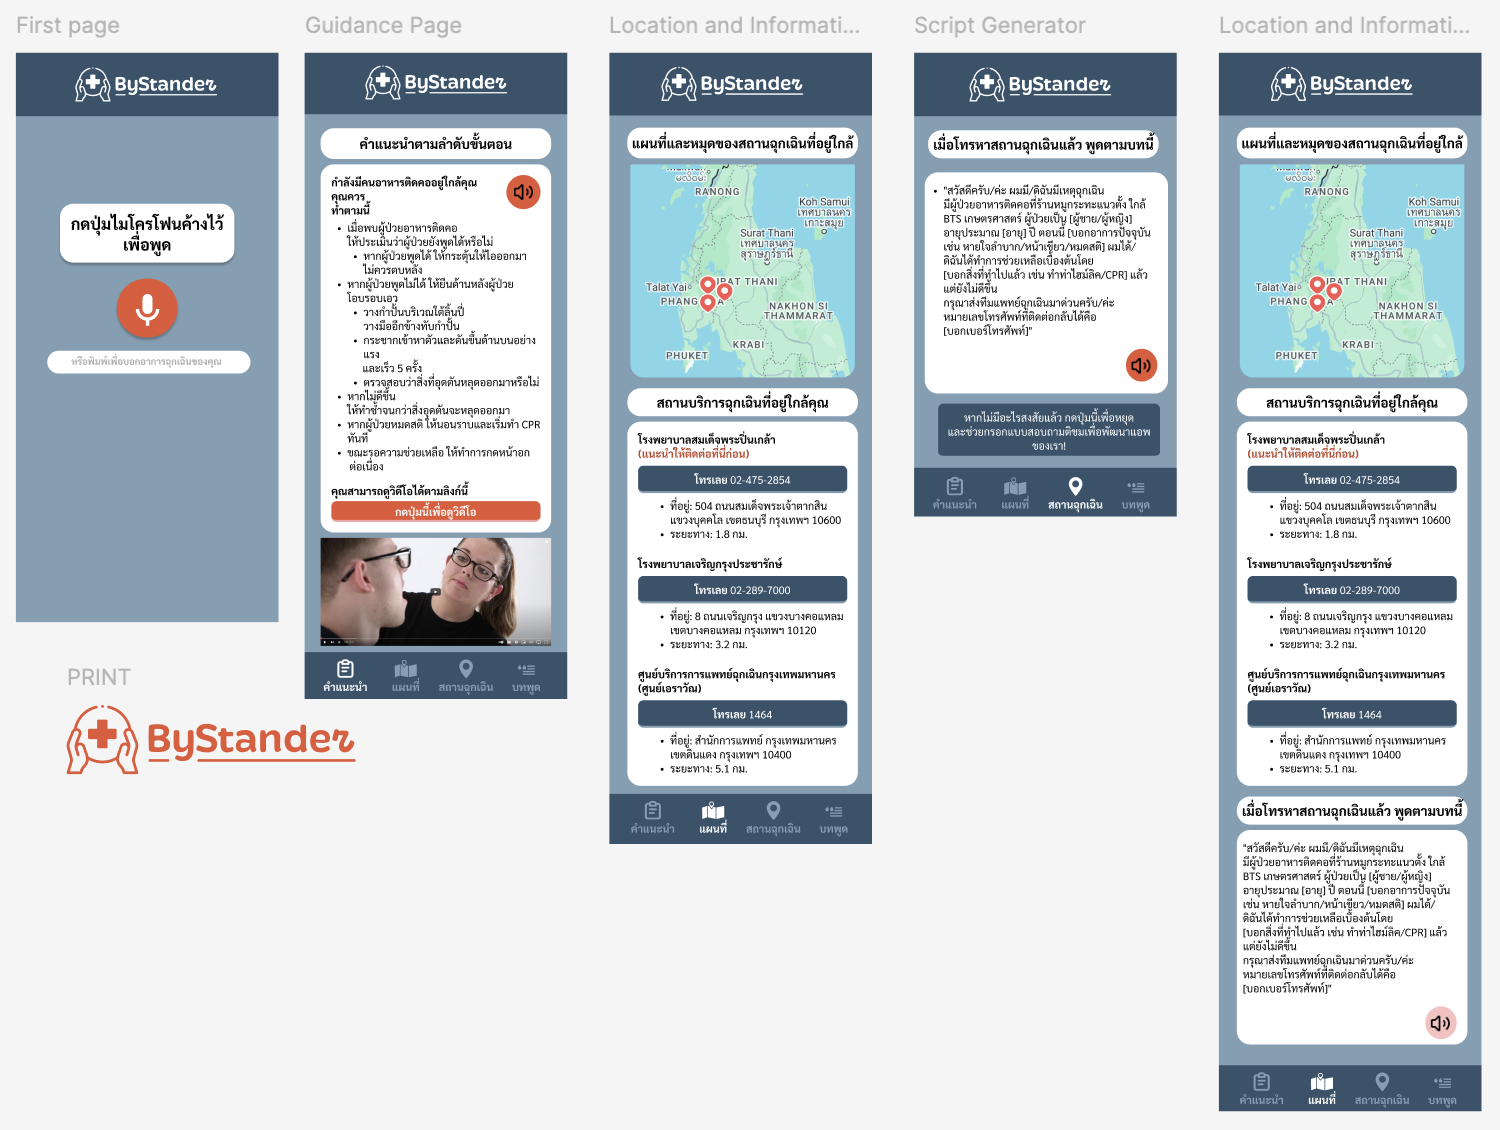
\includegraphics[width=0.9\textwidth]{/design/mockup-overall.png}
    \caption{Overall UI design of ByStander}
\end{figure}
\medskip % This \medskip separates the two figures and can remain.

\begin{figure}[h]
    \centering
    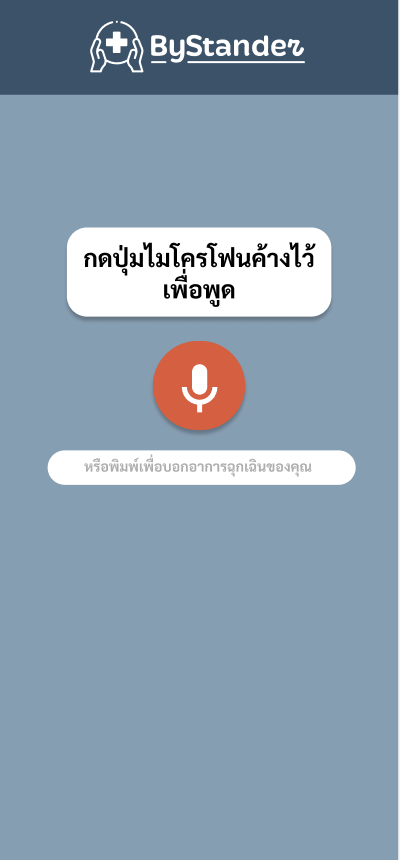
\includegraphics[width=0.2\textwidth]{/design/voice-detection.png}
    \caption{Emergency Voice Transcription Service UI}
\end{figure}
% The text block is now moved to be immediately after the figure environment above.
% The \medskip that was previously here (between this figure and the text) has been removed.
This is the UI design of the voice detection page. The user can press the button to start the voice detection and then the AI will transcribe the voice to text and show it on the screen. The user can also press the button again to stop the voice detection.
Or the user can type the text in the text box and then press the button to start the AI to generate the emergency guidance.
% If you need space after this paragraph before the next content, you can add \medskip or a blank line here.

\begin{figure}[h]
    \centering
    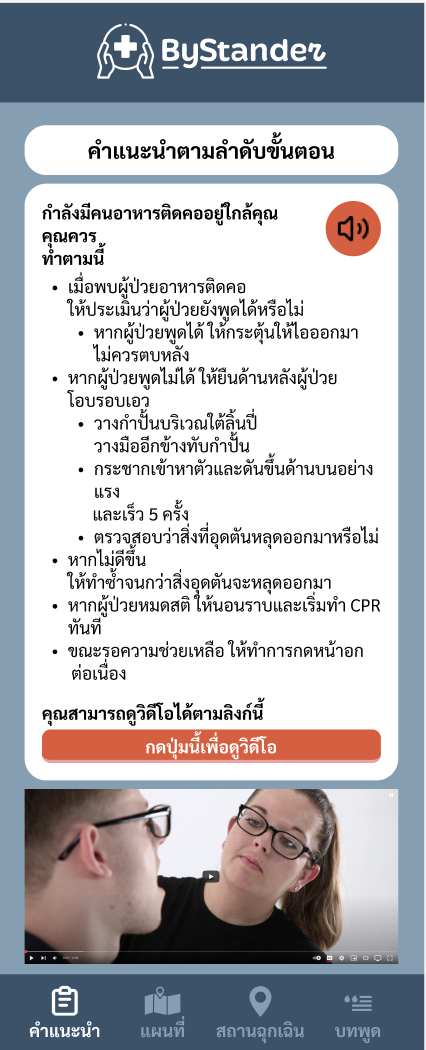
\includegraphics[width=0.2\textwidth]{/design/guidance-generation.png}
    \caption{Contextual Emergency Guidance Generation with Text-to-Speech for Guidance Service UI}
\end{figure}
This is the UI design of the contextual emergency guidance generation page. The user can see the emergency guidance and the video clip that is related to the emergency. 
The user can also press the button to listen to the guidance.

\begin{figure}[h]
    \centering
    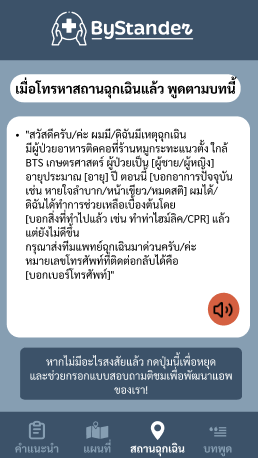
\includegraphics[width=0.2\textwidth]{/design/script-generator.png}
    \caption{Phone Operator Generation UI}
\end{figure}
This is the UI design of the phone operator generation page. The user can see the script that the AI generated for them to read to the operator. \\
\indent When the user is done with the process, they can press the button to complete and the app will direct user to the survey page.